\documentclass{beamer}
\usepackage{amsmath}
\usepackage{amsfonts}
\usepackage{amssymb}
\usepackage{polski}
\usepackage{pgfplots}
\pgfplotsset{compat=1.15}
\usepackage{mathrsfs}
\usepackage{wasysym}
\usepackage{booktabs}
\usetikzlibrary{arrows}
\usetheme{Warsaw}
\title{Ile ma Mach, czyli Falentyka}

\author{Franciszek Hansdorfer \and Jacek Winiarczyk}
\institute{Wydiział fizyki doświadczalnej instytutu Marii Mach}
\date{\today}
\begin{document}
\begin{frame}
\titlepage
\end{frame}

\begin{frame}{Co mogą zmierzyć mieszkańcy Falent?}
\begin{itemize}
\item $\pi$
\item $e$
\item Prędkość dźwięku w powietrzu ($1$ Mach)
\item Przenikalność magnetyczna próżni ($\epsilon_0$)
\item Przenikalność elektryczna próżni ($\mu_0$)
\item Stała Coulomba ($k_e$)
\item Prędkość światła ($c$)
\item Stała Plancka ($h$)
\item Zredukowana stała Plancka ($\hbar$)
\end{itemize}

\end{frame}

\section{Stałe matematyczne}

\subsection{$\pi$}

\begin{frame}{$\pi$ - igła Buffona}
$l$ - długość igły

$d$ - odległość między pionowymi liniami

$n$ - liczba rzutów

$R$ - liczba rzutów zakończonych przecięciem

$$p = \frac{2}{\pi} \frac{l}{d}$$
$$\frac{R}{n} = \frac{2}{\pi}\frac{l}{d}$$
$$\pi = \frac{2 l n}{d R}$$
$$\pi =$$

\end{frame}

\subsection{$e$}

\begin{frame}{$e$ - całkowanie gumką}

\end{frame}

\section{Parametry fizyczne}

\subsection{Prędkość dźwięku w powietrzu}

\begin{frame}{Prędkość dźwięku w powietrzu}
\begin{itemize}
\item Lab: [Zdjęcie Labu]
\item aparatura pomiarowa:
	\begin{itemize}
		\item Miarka $3$m
		\item Laptop Jacka
		\item Dłonie Franka
		\item Dłonie Jacka
		\item Termometr i higrometr
	\end{itemize}
\end{itemize}
[Zdjęcie eksperymentu]
\end{frame}

\begin{frame}{Dane}
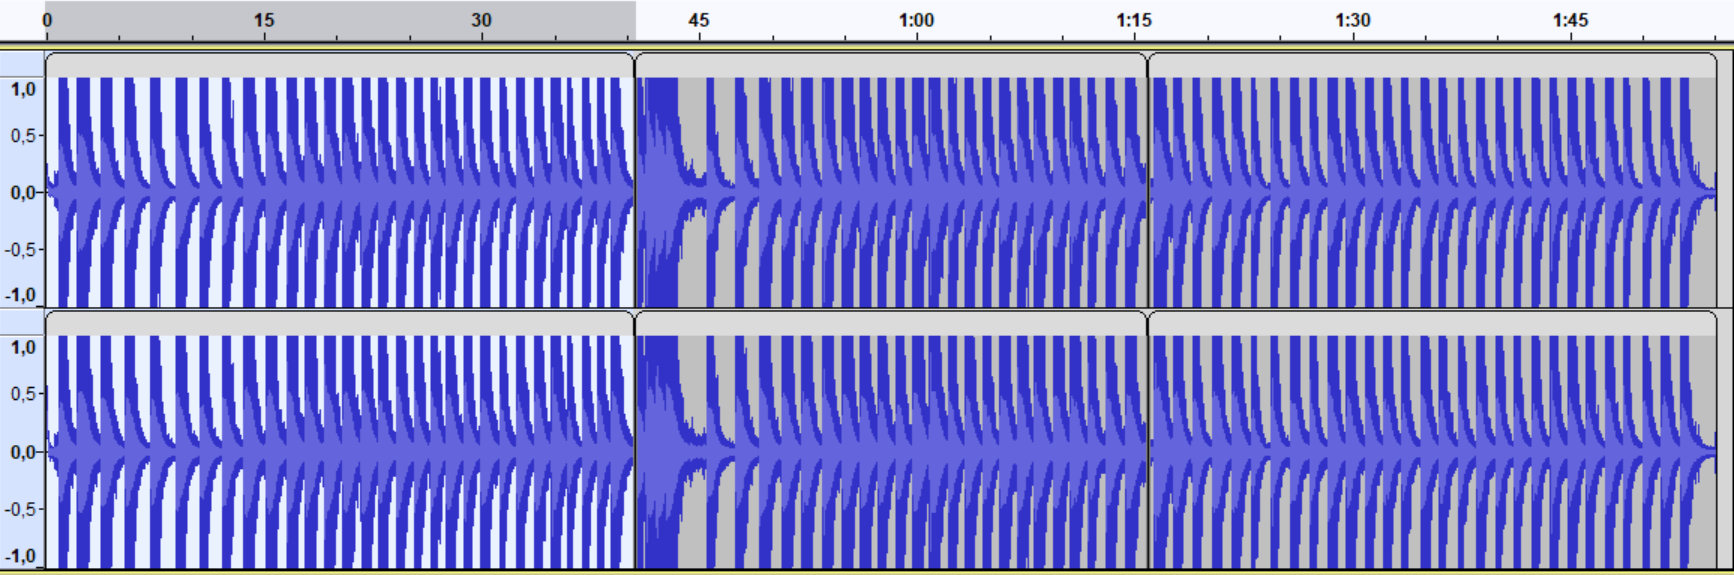
\includegraphics[width=\linewidth]{Data.png}
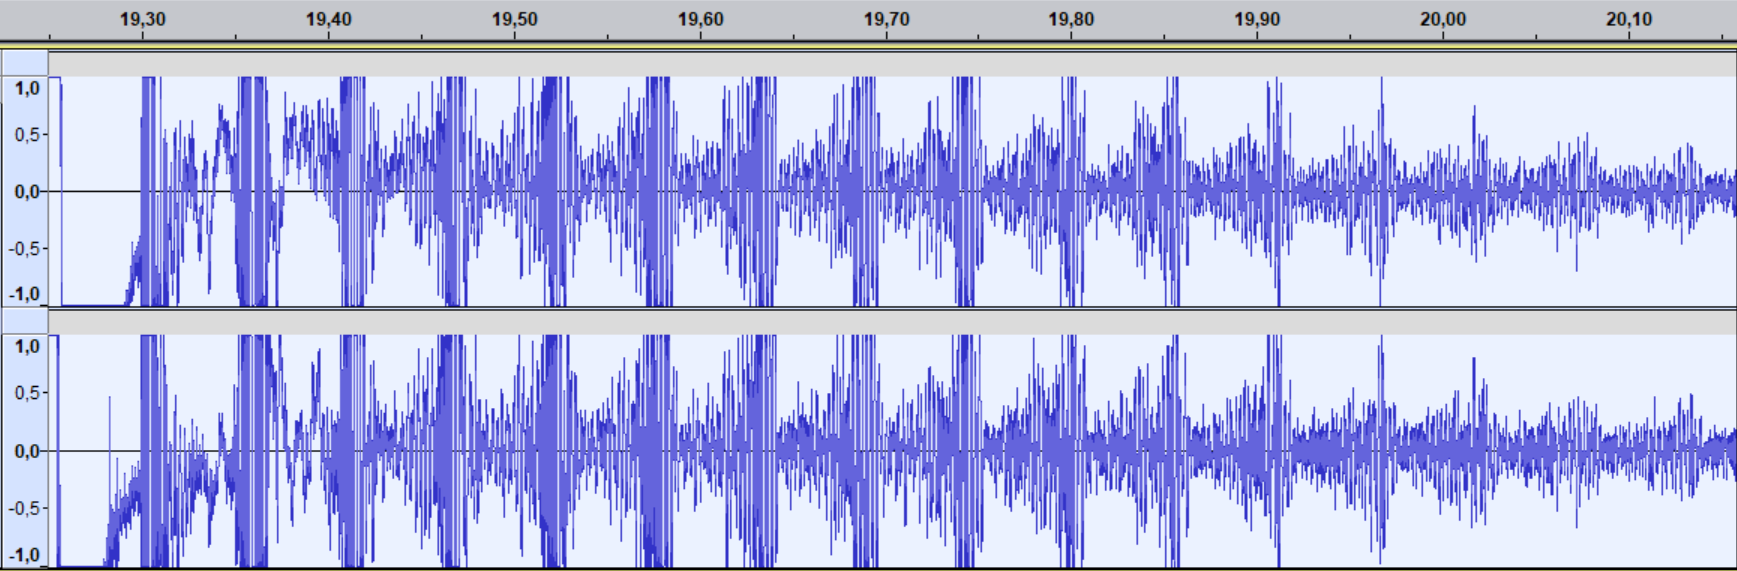
\includegraphics[width=\linewidth]{Data_zoom.png}
\end{frame}

\begin{frame}{Redukcja danych}
\centering
\begin{tabular}{cccc}
\toprule
Pomiar & czas [s] & sigma [s] & liczba pomiarów\\
\midrule
3 & 0.0534 & 0.00134 & 245 \\
4 & 0.0533 & 0.00127 & 117 \\
5 & 0.0544 & 0.00149 & 302 \\
6 & 0.0548 & 0.00180 & 688\\
7 & 0.0550 & 0.00119 & 762 \\
\bottomrule
\end{tabular}

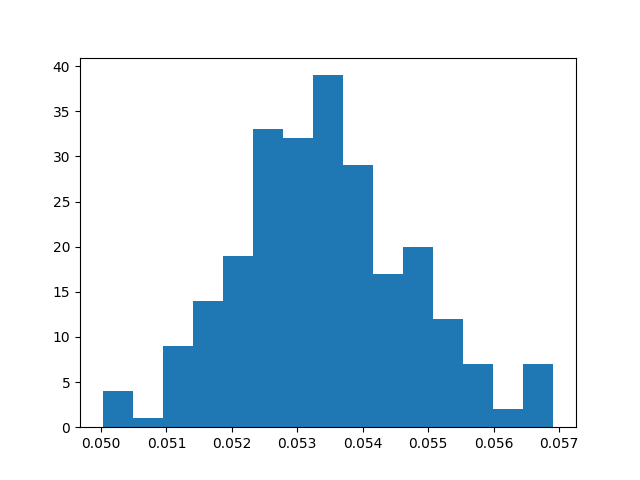
\includegraphics[width=0.2\linewidth]{Hist3.png}
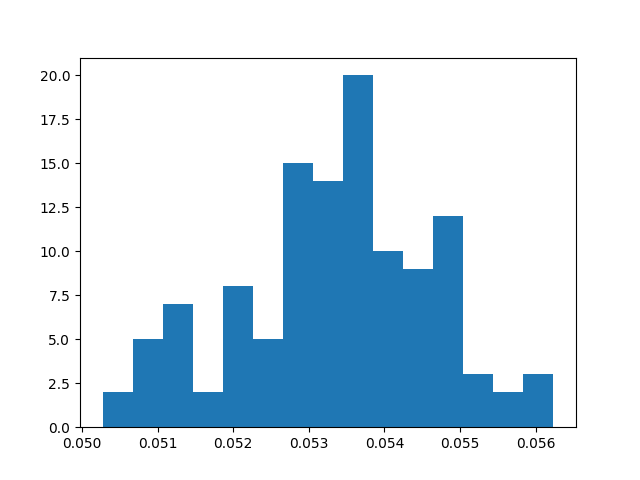
\includegraphics[width=0.2\linewidth]{Hist4.png}
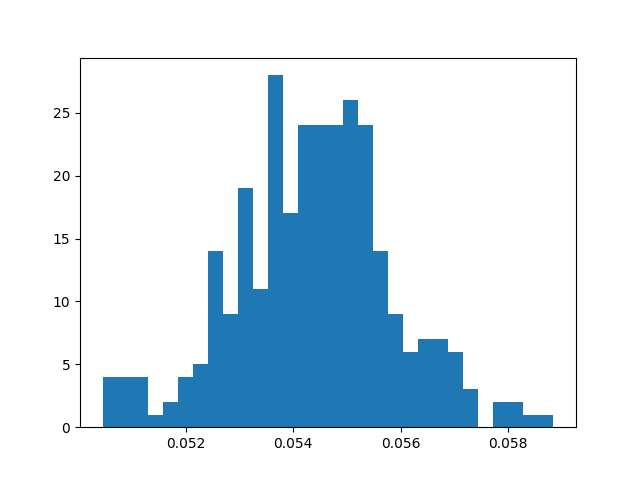
\includegraphics[width=0.2\linewidth]{Hist5.png}
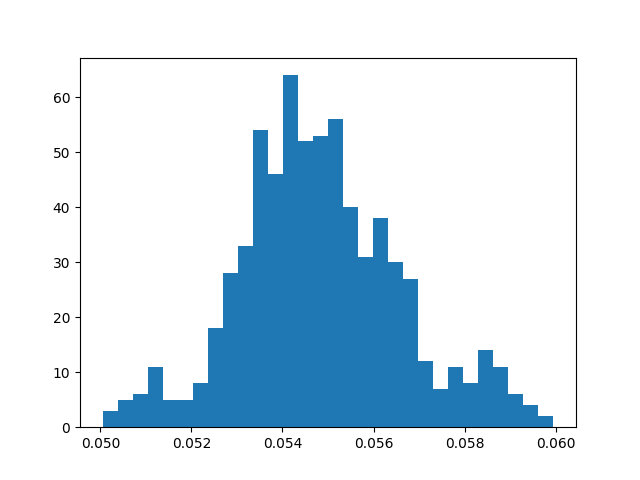
\includegraphics[width=0.2\linewidth]{Hist6.png}
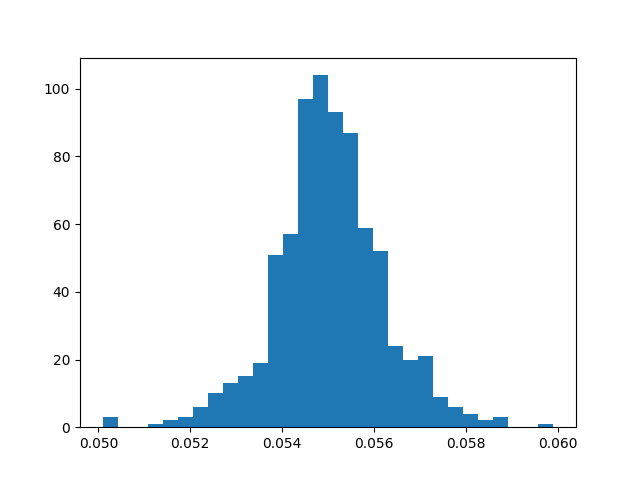
\includegraphics[width=0.2\linewidth]{Hist7.png}
\end{frame}

\begin{frame}{Wyniki i dyskusja błędu pomiarowego}
\centering
\begin{tabular}{cccc}
\toprule
Pomiar & temperatura [C] & wilgotność [\%]  & mach [m/s]\\
\midrule
3 & 29.12 & 27.83 & 355.71$\pm$8.90 \\
4 & 31.35 & 22.14 & 356.22$\pm$8.51 \\
5 & 20.22 & 44.42 & 349.41$\pm$9.57 \\
6 & 18.25 & 51.11 & 346.48$\pm$11.36 \\
7 & 18.22 & 51.53 & 345.19$\pm$7.46 \\
\bottomrule
\end{tabular}

\end{frame}

\begin{frame}{wyniki i dyskusja błędu pomiarowego}
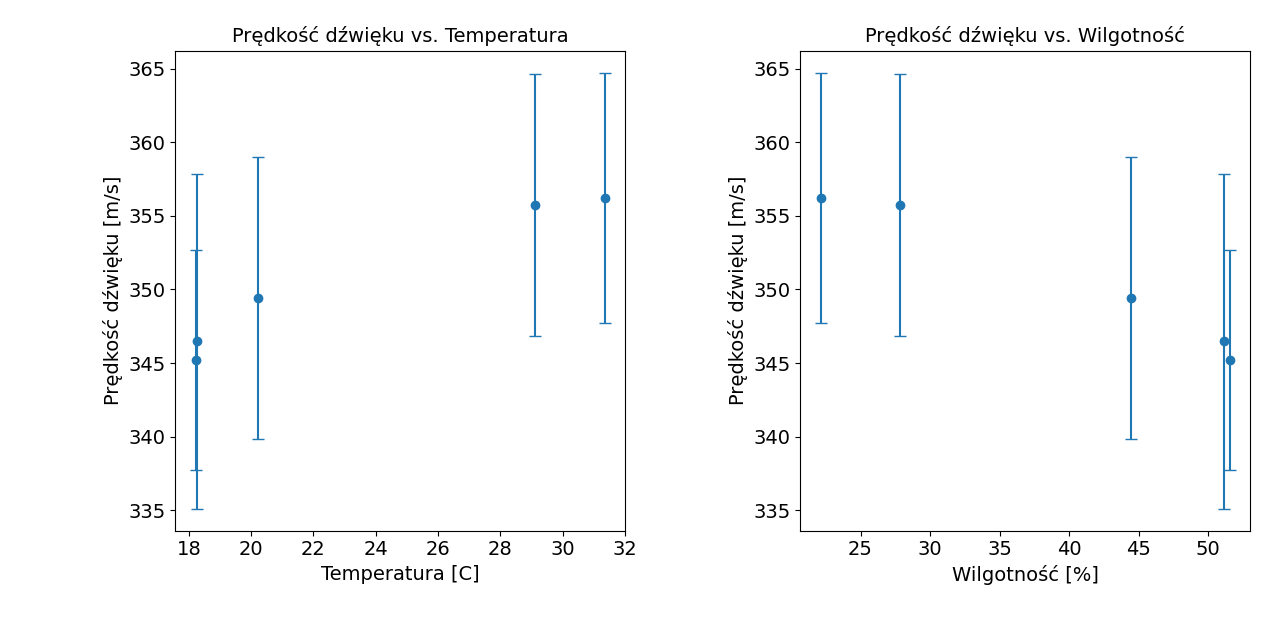
\includegraphics[width=\linewidth]{temp_humid_mach.png}

Prędkość dźwięku rośnie ze wzrostem temperatury i maleje wraz ze wzrostem wilgotności.
\end{frame}


\section{Stałe fizyczne}

\begin{frame}{Przenikalność magnetyczna próżni}

\end{frame}

\begin{frame}{Przenikalność elektryczna próżni}

\end{frame}

\begin{frame}{Stała Plancka}

\end{frame}


\section{Podsumowanie}

\begin{frame}{Dalsze kontynuacje badań}
\begin{itemize}
\item Stała Faradaya ($F$)
\item Ładunek elementarny ($e^-$)
\item Odległość Ziemia-Księżyc ($d_{\oplus - \leftmoon}$)
\item Promień Księżyca ($R_{\leftmoon}$)
\end{itemize}

\end{frame}



\end{document}